\label{ap:ap08}
\chapter{Aprendizado de máquina}
\section*{\textbf{A - ENUNCIADO}}
Para cada uma das tarefas abaixo (Classificação, Regressão etc.) e cada base de dados (Veículo, Diabetes etc.), fazer os
experimentos com todas as técnicas solicitadas (KNN, RNA etc.) e preencher os quadros com as estatísticas solicitadas,
bem como os resultados pedidos em cada experimento.

%%%%%%%%%%%%%%%%%%%%%%%%%%%%%%%%%%%%%%%%%%%%%%%%%%%%%%%%%%%%%%%%%%%%%%%%%%%%%%%%%%%%%%%%%%%%%
\section*{\textbf{B - RESOLUÇÃO}}
\begin{adjustwidth}{1em}{}
\textbf{Classificação}
\end{adjustwidth}

\begin{quote}
Para o experimento de Classificação:
\begin{itemize}
    \item Ordenar pela Acurácia (descendente), ou seja, a técnica de melhor
acurácia ficará em primeiro na tabela.
    \item Após o quadro colocar:
    \begin{itemize}
        \item Um resultado com 3 linhas com a predição de novos casos para a
técnica/parâmetro de maior Acurácia (criar um arquivo com novos casos à
sua escolha)
        \item A lista de comandos emitidos no RStudio para conseguir os resultados
obtidos
    \end{itemize}
\end{itemize}
\end{quote}

\begin{center}
    \textbf{Veículo}
\end{center}


\begin{longtable}{|>{\centering\arraybackslash}p{2.5cm}|>{\centering\arraybackslash}m{2.5cm}|c|m{7cm}|}
\caption{\mbox{Resultados da classificação na base de veículos}} \\
\hline
\textbf{Técnica} & \textbf{Parâmetro} & \textbf{Acurácia} & \textbf{Matriz de Confusão} \\
\hline
\endfirsthead

\hline
\textbf{Técnica} & \textbf{Parâmetro} & \textbf{Acurácia} & \textbf{Matriz de Confusão} \\
\hline
\endhead

\hline
\colorbox[HTML]{CAF2C2}{SVM - CV} & C=100 Sigma=0.015 & \colorbox[HTML]{CAF2C2}{0.8623} & 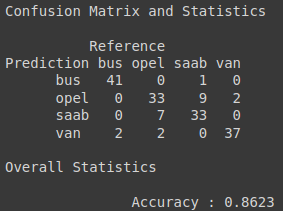
\includegraphics[width=0.4\textwidth]{apendices/fig/8_IAA008_1.png} \\
\hline
RNA - CV  & size=31 decay=0.4 & 0.8443 & 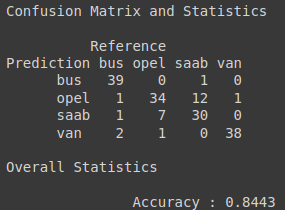
\includegraphics[width=0.4\textwidth]{apendices/fig/8_IAA008_2.png} \\
\hline
SVM - Hold-out  & C=1 Sigma= 0.0661018 & 0.7665 & 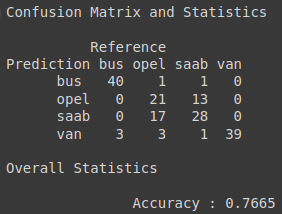
\includegraphics[width=0.4\textwidth]{apendices/fig/8_IAA008_3.png} \\
\hline
RF - CV   & mtry=5 & 0.7964 & 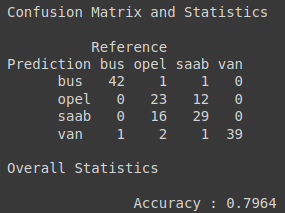
\includegraphics[width=0.4\textwidth]{apendices/fig/8_IAA008_4.png} \\
\hline
RF - Hold-out    & mtry=2 & 0.7844 & 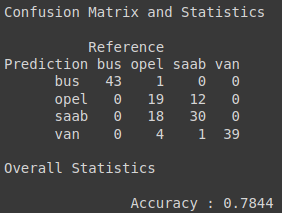
\includegraphics[width=0.4\textwidth]{apendices/fig/8_IAA008_5.png} \\
\hline
KNN    & k=3 & 0.7 & 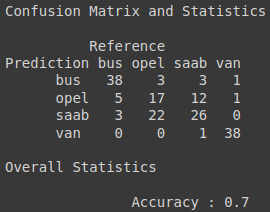
\includegraphics[width=0.4\textwidth]{apendices/fig/8_IAA008_6.png} \\
\hline
RNA - Hold-out    & size=3 decay=0.1 & 0.6287 & 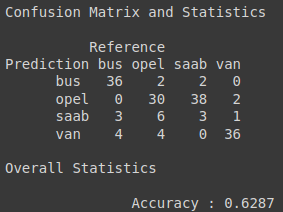
\includegraphics[width=0.4\textwidth]{apendices/fig/8_IAA008_7.png} \\
\hline
\end{longtable}


\begin{center}
    \textbf{Predição novos casos (SVM - CV)}
\end{center}

\begin{table}[H]
\caption{Resultados predição novos casos (SVM - CV) - Parte 1}
\hspace*{-1.5cm} % shift left (adjust as needed)
\begin{minipage}{\textwidth}
\centering
\begin{tabular}{|c|c|c|c|c|c|c|c|c|c|}
\hline
Comp & Circ & DCirc & RadRa & PrAxisRa & MaxLRa & ScatRa & Elong & PrAxisRect & MaxLRect \\
\hline
84   & 53   & 89    & 170   & 75       & 7      & 153    & 45    & 20         & 165 \\
\hline
87   & 35   & 90    & 450   & 57       & 8      & 160    & 50    & 15         & 165 \\
\hline
100  & 40   & 100   & 205   & 60       & 11     & 210    & 35    & 30         & 165 \\
\hline
\end{tabular}
\end{minipage}
\end{table}

\begin{table}[H]
\caption{Resultados predição novos casos (SVM - CV) - Parte 2 }
\hspace*{-2.5cm} % shift left (adjust as needed)
\begin{minipage}{\textwidth}
\centering
\begin{tabular}{|c|c|c|c|c|c|c|c|c|}
\hline
ScVarMaxis & ScVarmaxis & RaGyr & SkewMaxis & Skewmaxis & Kurtmaxis & KurtMaxis & HollRa & svm \\
\hline
170 & 350 & 180 & 65 & 8  & 15 & 180 & 197 & van \\
\hline
170 & 315 & 154 & 55 & 10 & 12 & 190 & 196 & opel \\
\hline
220 & 625 & 200 & 75 & 11 & 10 & 185 & 195 & saab \\
\hline
\end{tabular}
\end{minipage}
\end{table}


\begin{center}
    \textbf{Lista de comandos (SVM - CV)}
\end{center}

\begin{lstlisting}[language=R, style=input]
install.packages("e1071")
install.packages("caret")
install.packages("mlbench")
install.packages("mice")
install.packages("Metrics")
install.packages("kernlab")
library("caret")
library("mlbench")
library("mice")
library("Metrics")
setwd("/content")
seed_padrao <- 202412

dados <- read.csv("6 - Veiculos - Dados.csv")
dados$a <- NULL
View(dados)

set.seed(seed_padrao)
indices <- createDataPartition(dados$tipo, p=0.80, list=FALSE)
treino <- dados[indices,]
teste <- dados[-indices,]

ctrl <- trainControl(method = "cv", number = 10)
grid <- expand.grid(C=c(1, 2, 10, 50, 100), sigma=c(.01, .015,
0.2))
set.seed(seed_padrao)
svm <- train(form = tipo~. , data = treino , method = "svmRadial" ,
tuneGrid = grid , trControl = ctrl)
svm

predict.svm <- predict(svm, teste)
confusionMatrix(predict.svm, as.factor(teste$tipo))

dados_novos_casos <- read.csv("6 - Veiculos - Dados - Novos
Casos.csv")
dados_novos_casos$a <- NULL
View(dados_novos_casos)

predict.svm <- predict(svm, dados_novos_casos)
resultado <- cbind(dados_novos_casos, predict.svm)
resultado$tipo <- NULL
View(resultado)
\end{lstlisting}

\newpage
\begin{center}
    \textbf{Diabetes}
\end{center}


\begin{longtable}{|>{\centering\arraybackslash}p{3cm}|>{\centering\arraybackslash}m{2.5cm}|c|m{7cm}|}
\caption{\mbox{Resultados da classificação na base de diabetes}} \\
\hline
\textbf{Técnica} & \textbf{Parâmetro} & \textbf{Acurácia} & \textbf{Matriz de Confusão} \\
\hline
\endfirsthead

\hline
\textbf{Técnica} & \textbf{Parâmetro} & \textbf{Acurácia} & \textbf{Matriz de Confusão} \\
\hline
\endhead

\hline
\colorbox[HTML]{CAF2C2}{SVM Hold-out} & C=0.5 Sigma= 0.1219692 & \colorbox[HTML]{CAF2C2}{0.7843} & 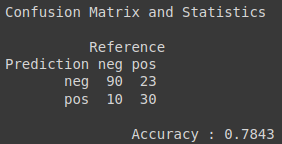
\includegraphics[width=0.4\textwidth]{apendices/fig/8_IAA008_8.png} \\
\hline
\colorbox[HTML]{CAF2C2}{SVM - CV} & C=0.5 Sigma= 0.1219692 & \colorbox[HTML]{CAF2C2}{0.7843} & 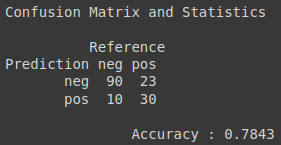
\includegraphics[width=0.4\textwidth]{apendices/fig/8_IAA008_9.png} \\
\hline
RNA - CV & size=11 decay=0.4 & 0.7778 & 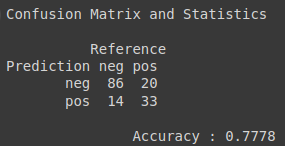
\includegraphics[width=0.4\textwidth]{apendices/fig/8_IAA008_10.png} \\
\hline
KNN & k=9 & 0.7727 & 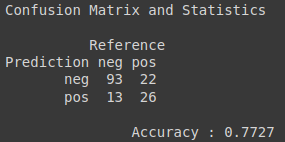
\includegraphics[width=0.4\textwidth]{apendices/fig/8_IAA008_11.png} \\
\hline
RF - Hold-out & mtry=2 & 0.7647 & 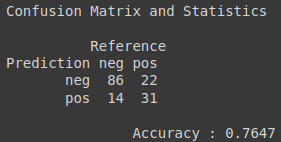
\includegraphics[width=0.4\textwidth]{apendices/fig/8_IAA008_12.png} \\
\hline
RF - CV  & mtry=8 & 0.7582 & 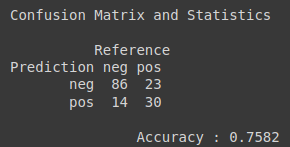
\includegraphics[width=0.4\textwidth]{apendices/fig/8_IAA008_13.png} \\
\hline
RNA Hold-out  & size=5 decay=0.1 & 0.7386 & 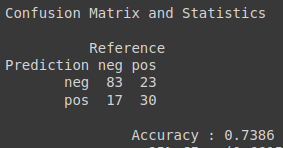
\includegraphics[width=0.4\textwidth]{apendices/fig/8_IAA008_14.png} \\
\hline
\end{longtable}


\begin{center}
    \textbf{Predição novos casos (SVM Hold-out)}
\end{center}

\begin{table}[H]
\centering
\caption{Resultados da predição novos casos (SVM Hold-out)}
\begin{tabular}{|c|c|c|c|c|c|c|c|c|}
\hline
preg0nt & glucose & pressure & triceps & insulin & mass & pedigree & age & predict.svm \\
\hline
8 & 140 & 80 & 30 & 0 & 40.5 & 500 & 45 & neg \\
\hline
8 & 120 & 50 & 40 & 0 & 20.7 & 625 & 35 & neg \\
\hline
2 & 50  & 60 & 25 & 0 & 30.3 & 544 & 32 & neg \\
\hline
\end{tabular}
\end{table}

\begin{center}
    \textbf{Lista de comandos (SVM Hold-out)}
\end{center}

\begin{lstlisting}[language=R, style=input]
install.packages("e1071")
install.packages("caret")
install.packages("mlbench")
install.packages("mice")
install.packages("Metrics")
install.packages("kernlab")
library("caret")
library("mlbench")
library("mice")
library("Metrics")

setwd("/content")
seed_padrao <- 202412

temp_dados <- read.csv("10 - Diabetes - Dados.csv")
temp_dados$num <- NULL
imp <- mice(temp_dados)
dados <- complete(imp, 1)
View(dados)

set.seed(seed_padrao)
indices <- createDataPartition(dados$diabetes, p=0.80,list=FALSE)
treino <- dados[indices,]
teste <- dados[-indices,]

set.seed(seed_padrao)
svm <- train(diabetes~., data=treino, method="svmRadial")
svm

predict.svm <- predict(svm, teste)
confusionMatrix(predict.svm, as.factor(teste$diabetes))

dados_novos_casos <- read.csv("10 - Diabetes - Dados - Novos
Casos.csv")
dados_novos_casos$num <- NULL
View(dados_novos_casos)

predict.svm <- predict(svm, dados_novos_casos)
resultado <- cbind(dados_novos_casos, predict.svm)
resultado$diabetes <- NULL
View(resultado)
\end{lstlisting}


\begin{adjustwidth}{1em}{}
\textbf{Regressão}
\end{adjustwidth}

\begin{quote}
Para o experimento de Regressão:
\begin{itemize}
    \item Ordenar por R2 descendente, ou seja, a técnica de melhor R2 ficará em primeiro na tabela.
    \item Após o quadro colocar:
    \begin{itemize}
        \item Um resultado com 3 linhas com a predição de novos casos para a técnica/parâmetro de maior R2 (criar um arquivo com novos casos à sua escolha)
        \item O Gráfico de Resíduos para a técnica/parâmetro de maior R2
        \item A lista de comandos emitidos no RStudio para conseguir os resultados obtidos
    \end{itemize}
\end{itemize}
\end{quote}

\newpage
\begin{center}
    \textbf{Admissão}
\end{center}


\begin{table}[H]
\caption{Resultados da regressão na base de admissão}
\hspace*{-1.5cm} 
\begin{minipage}{\textwidth}
\centering
{\renewcommand{\arraystretch}{1.7} % vertical padding
 %\setlength{\tabcolsep}{8pt}       % horizontal padding

\begin{tabular}{|c|p{3cm}|p{2cm}|p{2cm}|p{2cm}|p{2cm}|p{2cm}|}
\hline
\textbf{Técnica} & \textbf{Parâmetro} & \textbf{R2} & \textbf{Syx} & \textbf{Pearson} & \textbf{Rmse} & \textbf{MAE} \\
% \hline
% \colorbox[HTML]{CAF2C2}{SVM - CV} & C=2 Sigma=0.01 & \colorbox[HTML]{CAF2C2}{\makecell[l]{0.8882\\227024\\50831}} & \colorbox[HTML]{CAF2C2}{\makecell[l]{0.04632\\915579\\36475}} & \colorbox[HTML]{CAF2C2}{\makecell[l]{0.94268\\843613\\8658}} & \colorbox[HTML]{CAF2C2}{\makecell[l]{0.0441\\50573\\78381\\55}} & \colorbox[HTML]{CAF2C2}{\makecell[l]{0.0332\\09194\\19084\\42}} \\
% \hline
% SVM - Hold-out & C=1 Sigma= 0.2004666 & \makecell[l]{0.8676\\446382\\09649} & \makecell[l]{0.05041\\367457\\36519} & \makecell[l]{0.93174\\345191\\1874} & \makecell[l]{0.0480\\43022\\17141\\79} & \makecell[l]{0.0362\\44211\\18180\\7} \\
% \hline
% RF - Hold-out  & mtry=2 & \makecell[l]{0.8609\\300253\\48176} & \makecell[l]{0.05167\\664040\\73779} & \makecell[l]{0.93087\\499063\\6073} & \makecell[l]{0.0492\\46598\\30556\\37} & \makecell[l]{0.0368\\19141\\50290\\51} \\
% \hline
% RF - CV  & mtry=2 & \makecell[l]{0.8609\\300253\\48176} & \makecell[l]{0.05167\\664040\\73779} & \makecell[l]{0.93087\\499063\\6073} & \makecell[l]{0.0492\\46598\\30556\\37} & \makecell[l]{0.0368\\19141\\50290\\51} \\
% \hline
% RNA - CV  & size=5 decay=0.1 & \makecell[l]{0.8391\\787415\\23624} & \makecell[l]{0.05557\\114075\\7806} & \makecell[l]{0.91931\\808890\\1637} & \makecell[l]{0.0529\\57963\\68935\\19} & \makecell[l]{0.0435\\61868\\14603\\77} \\
% \hline
% RNA - Hold-out  & size=5 decay=0.1 & \makecell[l]{0.8293\\968576\\03891} & \makecell[l]{0.05723\\624012\\77942} & \makecell[l]{0.91489\\468169\\6537} & \makecell[l]{0.0545\\44763\\43419\\27} & \makecell[l]{0.0454\\27406\\52315\\09} \\
% \hline
% KNN  & K=9  & \makecell[l]{0.7773\\387140\\24105} & \makecell[l]{0.06538\\828402\\4072} & \makecell[l]{0.88345\\699730\\2136} & \makecell[l]{0.0623\\13465\\65563\\19} & \makecell[l]{0.0481\\85941\\04308\\39} \\
\hline%%%%%%%%%%%%%%%%%%%%%%%%%%%%%%%%%%%%%
\colorbox[HTML]{CAF2C2}{SVM - CV} & C=2 Sigma=0.01 & \colorbox[HTML]{CAF2C2}{0.8882} & \colorbox[HTML]{CAF2C2}{0.0463} & \colorbox[HTML]{CAF2C2}{0.9427} & \colorbox[HTML]{CAF2C2}{0.0442} & \colorbox[HTML]{CAF2C2}{0.0332} \\
\hline
SVM - Hold-out & C=1 Sigma= 0.2004666 & 0.8676 & 0.0504 & 0.9317 & 0.0480 & 0.0362 \\
\hline
RF - Hold-out & mtry=2 & 0.8609 & 0.0517 & 0.9309 & 0.0492 & 0.0368 \\
\hline
RF - CV & mtry=2 & 0.8609 & 0.0517 & 0.9309 & 0.0492 & 0.0368 \\
\hline
RNA - CV & \makecell[l]{size=5\\decay=0.1} & 0.8392 & 0.0556 & 0.9193 & 0.0529 & 0.0436 \\
\hline
RNA - Hold-out & \makecell[l]{size=5\\decay=0.1} & 0.8294 & 0.0572 & 0.9149 & 0.0545 & 0.0454 \\
\hline
KNN & K=9 & 0.7773 & 0.0654 & 0.8835 & 0.0623 & 0.0482 \\
\hline
\end{tabular}
}
\end{minipage}
\end{table}


\begin{center}
    \textbf{Predição novos casos (SVM - CV)}
\end{center}

\begin{table}[H]
\centering
\caption{Resultados da predição novos casos (SVM - CV)}
\begin{tabular}{|c|c|c|c|c|c|c|c|}
\hline
GRE.S & TOEFL.S & University.R & SOP & LOR & CGPA & Research & predict \\
\hline
300 & 125 & 3 & 4.5 & 4.5 & 8.87 & 1 & 0.7948 \\
\hline
350 & 99 & 4 & 3.0 & 3.0 & 9.00 & 1 & 0.8113 \\
\hline
325 & 85 & 4 & 4.5 & 3.5 & 8.75 & 1 & 0.7042 \\
\hline
\end{tabular}
\end{table}


\begin{center}
    \textbf{Gráfico de resíduos (SVM - CV)}
\end{center}

\begin{figure}[H]
\centering
\caption{Gráfico de resíduos (SVM - CV)}
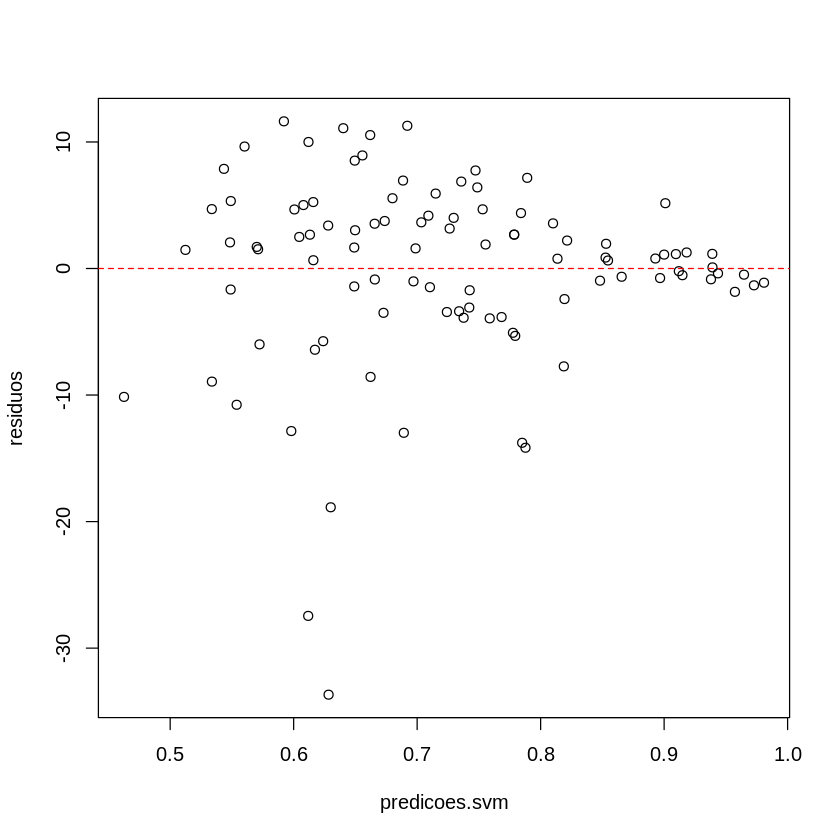
\includegraphics[width=.8\linewidth]{apendices/fig/8_IAA008_15.png}
\end{figure}

\begin{center}
    \textbf{Lista de comandos (SVM – CV)}
\end{center}


\begin{lstlisting}[language=R, style=input]
install.packages("e1071")
install.packages("caret")
install.packages("mlbench")
install.packages("mice")
install.packages("Metrics")
install.packages("kernlab")
library("caret")
library("mlbench")
library("mice")
library("Metrics")

setwd("/content")
seed_padrao <- 202412

dados <- read.csv("9 - Admissao - Dados.csv", header=T)
dados$num <- NULL
View(dados)

set.seed(seed_padrao)
indices <- createDataPartition(dados$ChanceOfAdmit, p=0.80,
list=FALSE)
treino <- dados[indices,]
teste <- dados[-indices,]

control <- trainControl(method = "cv", number = 10)
tuneGrid <- expand.grid(C=c(1, 2, 10, 50, 100), sigma=c(.01, .015,
0.2))
set.seed(seed_padrao)
svm <- train(ChanceOfAdmit~., data=treino, method="svmRadial",
trainControl=control, tuneGrid=tuneGrid)
svm
predicoes.svm <- predict(svm, teste)

print("RMSE")
rmse(teste$ChanceOfAdmit, predicoes.svm)

print("R2")
r2 <- function(predito, observado) {
return(1 - (sum((predito-observado)^2) /
sum((observado-mean(observado))^2)))
}
r2(predicoes.svm,teste$ChanceOfAdmit)

print("SYX")
syx <- function(predito, observado, n, p)
{
sqrt((sum((observado-predito)^2))/(n-p-1))
}
syx(predicoes.svm,teste$ChanceOfAdmit, nrow(teste), ncol(teste))

print("PEARSON")
pearson <- function(predito, observado) {
n <- length(predito)
predito_media <- mean(predito)
observado_media <- mean(observado)

num <- sum((predito - predito_media) * (observado -
observado_media))
denom <- sqrt(sum((predito - predito_media)^2) * sum((observado -
observado_media)^2))

r <- num / denom
return(r)
}
pearson(predicoes.svm, teste$ChanceOfAdmit)

print("MAE")
mae <- function(predito, observado)
{
error = observado-predito
mean(abs(error))
}
mae(predicoes.svm, teste$ChanceOfAdmit)

residuos <- ((teste$ChanceOfAdmit -
predicoes.svm)/teste$ChanceOfAdmit)*100
plot(residuos ~ predicoes.svm)
abline(h = 0, lty = 2, col = "red")

dados_novos_casos <- read.csv("9 - Admissao - Dados - Novos
Casos.csv")
dados_novos_casos$num <- NULL
View(dados_novos_casos)

predict.svm <- predict(svm, dados_novos_casos)
resultado <- cbind(dados_novos_casos, predict.svm)
resultado$ChanceOfAdmit <- NULL
View(resultado)
\end{lstlisting}


\begin{center}
    \textbf{Biomassa}
\end{center}

% \begin{table}[H]
% \centering
% \caption{Resultados da regressão na base de biomassa}
% \hspace*{-3cm} % shift left (adjust as needed)
% \begin{minipage}{\textwidth}
% \begin{tabular}{|l|l|l|l|l|l|l|}
% \hline
% \textbf{Técnica} & \textbf{Parâmetro} & \textbf{R$^2$} & \textbf{Syx} & \textbf{Pearson} & \textbf{RMSE} & \textbf{MAE} \\
% \hline
% \colorbox[HTML]{CAF2C2}{RNA CV} & \makecell[l]{size=3\\decay=0.1} & \colorbox[HTML]{CAF2C2}{0.9051} & \colorbox[HTML]{CAF2C2}{821702.3177} & \colorbox[HTML]{CAF2C2}{0.9882} & \colorbox[HTML]{CAF2C2}{800372.9388} & \colorbox[HTML]{CAF2C2}{369.3600} \\
% \hline
% RNA Hold-out & \makecell[l]{size=3\\decay=0.1} & 0.8993 & 425162.0640 & 0.9751 & 215677.6934 & 380.5700 \\
% \hline
% RF Hold-out & mtry=2 & 0.8869 & 383207.4007 & 0.9852 & 47347.9748 & 403.3300 \\
% \hline
% RF CV & mtry=2 & 0.8869 & 383207.4007 & 0.9852 & 47347.9748 & 403.3300 \\
% \hline
% SVM CV & \makecell[l]{C=100\\Sigma=0.01} & 0.8091 & 401908.7333 & 0.9605 & 377289.1498 & 524.0400 \\
% \hline
% KNN & K=1 & 0.7776 & 938518.5302 & 0.9471 & 90255.5295 & 565.5700 \\
% \hline
% SVM Hold-out & \makecell[l]{C=1\\Sigma=0.8644} & 0.4750 & 264957.0777 & 0.8535 & 943243.0766 & 869.1200 \\
% \hline
% \end{tabular}
% \end{minipage}
% \end{table}
\begin{table}[H]
\caption{Resultados da regressão na base de biomassa}
\hspace*{-1.5cm} 
\begin{minipage}{\textwidth}
\centering
{\renewcommand{\arraystretch}{1.7} % vertical padding
 %\setlength{\tabcolsep}{8pt}       % horizontal padding

\begin{tabular}{|c|p{3cm}|p{2cm}|p{2cm}|p{2cm}|p{2cm}|p{2cm}|}
\hline
\textbf{Técnica} & \textbf{Parâmetro} & \textbf{R$^2$} & \textbf{Syx} & \textbf{Pearson} & \textbf{RMSE} & \textbf{MAE} \\
\hline
\colorbox[HTML]{CAF2C2}{RNA CV} & \makecell[l]{size=3\\decay=0.1} & \colorbox[HTML]{CAF2C2}{0.9051} & \colorbox[HTML]{CAF2C2}{385.7903} & \colorbox[HTML]{CAF2C2}{0.9882} & \colorbox[HTML]{CAF2C2}{369.3660} & 109.9805 \\
\hline
RNA Hold-out & \makecell[l]{size=3\\decay=0.1} & 0.8993 & 397.4928 & 0.9751 & 380.5704 & 256.7893 \\
\hline
RF Hold-out & mtry=2 & 0.8869 & 421.2733 & 0.9852 & 403.3385 & \colorbox[HTML]{CAF2C2}{102.0527} \\
\hline
RF CV & mtry=2 & 0.8869 & 421.2733 & 0.9852 & 403.3385 & \colorbox[HTML]{CAF2C2}{102.0527} \\
\hline
SVM CV & \makecell[l]{C=100\\Sigma=0.01} & 0.8091 & 547.3479 & 0.9605 & 524.0457 & 154.5247 \\
\hline
KNN & K=1 & 0.7776 & 590.7204 & 0.9471 & 565.5717 & 128.5157 \\
\hline
SVM Hold-out & \makecell[l]{C=1\\Sigma=0.8644} & 0.4750 & 907.7681 & 0.8535 & 869.1218 & 199.1633 \\
\hline
\end{tabular}
}
\end{minipage}
\end{table}



\begin{center}
    \textbf{Predição novos casos (RNA - CV)}
\end{center}

\begin{table}[H]
\centering
\caption{Resultado da predição novos casos (RNA - CV)}
\begin{tabular}{|r|r|r|r|}
\hline
dap & h & Me & predict.rna \\
\hline
7.0 & 4.0 & 1.04 & 82.9916 \\
\hline
8.2 & 6.0 & 1.04 & 109.7899 \\
\hline
7.5 & 5.5 & 1.04 & 98.4963 \\
\hline
\end{tabular}
\end{table}


\begin{center}
    \textbf{Gráfico de resíduos (RNA – CV)}
\end{center}


\begin{figure}[H]
\centering
\caption{Gráfico de resíduos (RNA - CV)}
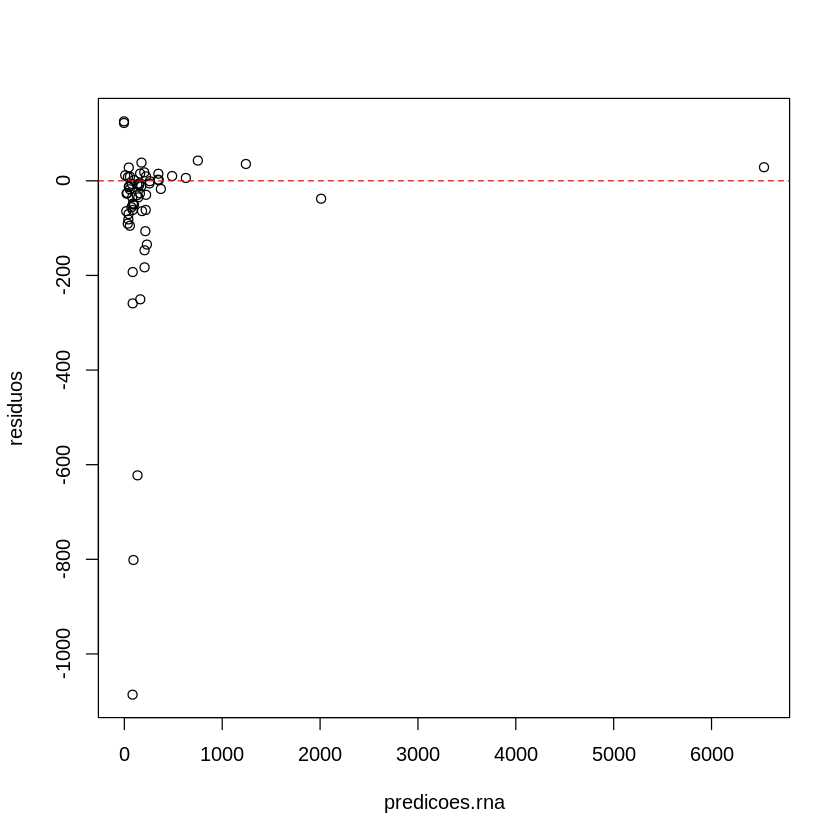
\includegraphics[width=.8\linewidth]{apendices/fig/8_IAA008_16.png}
\end{figure}



\begin{center}
    \textbf{Lista de comandos (RNA - CV)}
\end{center}



\begin{lstlisting}[language=R, style=input]
install.packages("e1071")
install.packages("caret")
install.packages("mlbench")
install.packages("mice")
install.packages("Metrics")
library("caret")
library("mlbench")
library("mice")
library("Metrics")

setwd("/content")
seed_padrao <- 202412

dados <- read.csv("5 - Biomassa - Dados.csv")
View(dados)

set.seed(seed_padrao)
ind <- createDataPartition(dados$biomassa, p=0.80, list = FALSE)
treino <- dados[ind,]
teste <- dados[-ind,]

control <- trainControl(method = "cv", number = 10)
set.seed(seed_padrao)
rna <- train(biomassa~., data=treino, method="nnet",
trainControl=control, linout=T, MaxNWts=10000, maxit=2000, trace=F)
rna
predicoes.rna <- predict(rna, teste)

print("RMSE")
rmse(teste$biomassa, predicoes.rna)

print("R2")
r2 <- function(predito, observado) {
return(1 - (sum((predito-observado)^2) /
sum((observado-mean(observado))^2)))
}
r2(predicoes.rna,teste$biomassa)

print("SYX")
syx <- function(predito, observado, n, p)
{
sqrt((sum((observado-predito)^2))/(n-p-1))
}
syx(predicoes.rna,teste$biomassa, nrow(teste), ncol(teste))

print("PEARSON")
pearson <- function(predito, observado) {
n <- length(predito)
predito_media <- mean(predito)
observado_media <- mean(observado)

num <- sum((predito - predito_media) * (observado -
observado_media))
denom <- sqrt(sum((predito - predito_media)^2) * sum((observado -
observado_media)^2))

r <- num / denom
return(r)
}
pearson(predicoes.rna, teste$biomassa)

print("MAE")
mae <- function(predito, observado)
{
error = observado-predito
mean(abs(error))
}
mae(predicoes.rna, teste$biomassa)

residuos <- ((teste$biomassa - predicoes.rna)/teste$biomassa)*100
plot(residuos ~ predicoes.rna)
abline(h = 0, lty = 2, col = "red")

dados_novos_casos <- read.csv("5 - Biomassa - Dados - Novos
Casos.csv")
View(dados_novos_casos)

predict.rna <- predict(rna, dados_novos_casos)
resultado <- cbind(dados_novos_casos, predict.rna)
resultado$biomassa <- NULL
View(resultado)
\end{lstlisting}


\begin{adjustwidth}{1em}{}
\textbf{Agrupamento}
\end{adjustwidth}

\begin{center}
    \textbf{Veículo}
\end{center}

% --- Parte 1 ---
\begin{table}[H]
\centering
\caption{Clusters gerados - Parte 1}
\begin{tabular}{|c|c|c|c|c|c|c|c|}
\hline
Cluster & Comp & Circ & DCirc & Rad & Ra & PraxisRa & MaxLRa \\ \hline
1  & 85  & 43  & 70  & 120 & 56 & 7  & 149 \\ \hline
2  & 104 & 54  & 101 & 189 & 57 & 11 & 222 \\ \hline
3  & 89  & 45  & 72  & 166 & 59 & 7  & 154 \\ \hline
4  & 89  & 41  & 66  & 162 & 58 & 7  & 150 \\ \hline
5  & 90  & 37  & 74  & 169 & 59 & 7  & 157 \\ \hline
6  & 88  & 40  & 69  & 146 & 58 & 9  & 133 \\ \hline
7  & 101 & 53  & 108 & 197 & 60 & 11 & 214 \\ \hline
8  & 93  & 39  & 66  & 133 & 59 & 8  & 130 \\ \hline
9  & 85  & 36  & 51  & 116 & 57 & 6  & 122 \\ \hline
10 & 100 & 47  & 105 & 209 & 64 & 10 & 201 \\ \hline
\end{tabular}
\end{table}

% --- Parte 2 ---
\begin{table}[H]
\centering
\caption{Clusters gerados - Parte 2}
\begin{tabular}{|c|c|c|c|c|c|c|c|}
\hline
Cluster & ScatRa & Elong & PraxisRect & MaxLRect & ScVarMaxis & ScVarmxis & RaGyr \\ \hline
1  & 45 & 19 & 143 & 170 & 327 & 171 & 81 \\ \hline
2  & 30 & 25 & 173 & 225 & 706 & 216 & 72 \\ \hline
3  & 44 & 19 & 144 & 174 & 347 & 174 & 69 \\ \hline
4  & 45 & 19 & 144 & 169 & 331 & 161 & 64 \\ \hline
5  & 43 & 20 & 131 & 189 & 363 & 186 & 72 \\ \hline
6  & 50 & 18 & 135 & 202 & 259 & 151 & 66 \\ \hline
7  & 31 & 24 & 162 & 226 & 661 & 214 & 71 \\ \hline
8  & 52 & 18 & 134 & 159 & 246 & 139 & 63 \\ \hline
9  & 57 & 17 & 125 & 137 & 196 & 123 & 85 \\ \hline
10 & 33 & 23 & 147 & 214 & 586 & 201 & 67 \\ \hline
\end{tabular}
\end{table}

% --- Parte 3 ---
\begin{table}[H]
\centering
\caption{Clusters gerados - Parte 3}
\begin{tabular}{|c|c|c|c|c|c|}
\hline
Cluster & SkewMaxis & Skewmaxis & Kurtmaxis & KurtMaxis & Tipo \\ \hline
1  & 6  & 11 & 180 & 184 & bus  \\ \hline
2  & 0  & 11 & 187 & 198 & opel \\ \hline
3  & 5  & 2  & 190 & 196 & opel \\ \hline
4  & 4  & 0  & 188 & 197 & van  \\ \hline
5  & 1  & 7  & 196 & 202 & bus  \\ \hline
6  & 0  & 21 & 193 & 200 & opel \\ \hline
7  & 0  & 24 & 188 & 199 & saab \\ \hline
8  & 5  & 7  & 183 & 194 & van  \\ \hline
9  & 1  & 5  & 180 & 183 & saab \\ \hline
10 & 2  & 13 & 192 & 198 & bus  \\ \hline
\end{tabular}
\end{table}

10 primeiras linhas do arquivo com o cluster correspondente:

% --- Parte 1 ---
\begin{table}[H]
\centering
\caption{Resumo do cluster correspondente - Parte 1}
\begin{tabular}{|c|c|c|c|c|c|c|c|}
\hline
Cluster & Comp & Circ & DCirc & Rad & Ra & PraxisRa & MaxLRa \\ \hline
4  & 95  & 48  & 83  & 178 & 72  & 10 & 162 \\ \hline
1  & 91  & 41  & 84  & 141 & 57  & 9  & 149 \\ \hline
10 & 104 & 50  & 106 & 209 & 66  & 10 & 207 \\ \hline
4  & 93  & 41  & 82  & 159 & 63  & 9  & 144 \\ \hline
1  & 85  & 44  & 70  & 205 & 103 & 52 & 149 \\ \hline
9  & 107 & 57  & 106 & 172 & 50  & 6  & 255 \\ \hline
1  & 97  & 43  & 73  & 173 & 65  & 6  & 153 \\ \hline
8  & 90  & 43  & 66  & 157 & 65  & 9  & 137 \\ \hline
9  & 86  & 34  & 62  & 140 & 61  & 7  & 122 \\ \hline
7  & 93  & 44  & 98  & 197 & 62  & 11 & 183 \\ \hline
\end{tabular}
\end{table}

% --- Parte 2 ---
\begin{table}[H]
\centering
\caption{Resumo do cluster correspondente - Parte 2}
\begin{tabular}{|c|c|c|c|c|c|c|c|}
\hline
Cluster & ScatRa & Elong & PraxisRect & MaxLRect & ScVarMaxis & ScVarmxis & RaGyr \\ \hline
4  & 42 & 20 & 159 & 176 & 379 & 184 & 70 \\ \hline
1  & 45 & 19 & 143 & 170 & 330 & 158 & 72 \\ \hline
10 & 32 & 23 & 158 & 223 & 635 & 220 & 73 \\ \hline
4  & 46 & 19 & 143 & 160 & 309 & 127 & 63 \\ \hline
1  & 45 & 19 & 144 & 241 & 325 & 188 & 127 \\ \hline
9  & 26 & 28 & 169 & 280 & 957 & 264 & 85 \\ \hline
1  & 42 & 19 & 143 & 176 & 361 & 172 & 66 \\ \hline
8  & 48 & 18 & 146 & 162 & 281 & 164 & 67 \\ \hline
9  & 54 & 17 & 127 & 141 & 223 & 112 & 64 \\ \hline
7  & 36 & 22 & 146 & 202 & 505 & 152 & 64 \\ \hline
\end{tabular}
\end{table}

% --- Parte 3 ---
\begin{table}[H]
\centering
\caption{Resumo do cluster correspondente - Parte 3}
\begin{tabular}{|c|c|c|c|c|c|}
\hline
Cluster & SkewMaxis & Skewmaxis & Kurtmaxis & KurtMaxis & Tipo \\ \hline
4  & 6  & 16 & 187 & 197 & van  \\ \hline
1  & 9  & 14 & 189 & 199 & van  \\ \hline
10 & 14 & 9  & 188 & 196 & saab \\ \hline
4  & 6  & 10 & 199 & 207 & van  \\ \hline
1  & 9  & 11 & 180 & 183 & bus  \\ \hline
9  & 5  & 9  & 181 & 183 & bus  \\ \hline
1  & 13 & 1  & 200 & 204 & bus  \\ \hline
8  & 3  & 3  & 193 & 202 & van  \\ \hline
9  & 2  & 14 & 200 & 208 & van  \\ \hline
7  & 4  & 14 & 195 & 204 & saab \\ \hline
\end{tabular}
\end{table}



\begin{center}
    \textbf{Lista de comandos emitidos}
\end{center}


\begin{lstlisting}[language=R, style=input]
install.packages("klaR")
library(klaR)

setwd("/content")
seed_padrao <- 202412

dados <- read.csv("6 - Veiculos - Dados.csv")
dados$a <- NULL
View(dados)

set.seed(seed_padrao)
cluster.results <- kmodes(dados, 10, iter.max = 10, weighted =
FALSE )
cluster.results

resultado <- cbind(dados, cluster.results$cluster)
resultado
\end{lstlisting}


\begin{adjustwidth}{1em}{}
\textbf{Regras de associação}
\end{adjustwidth}

\begin{center}
    \textbf{Musculação}
\end{center}

Regras geradas com uma configuração de Suporte e Confiança.


\begin{figure}[H]
\centering
\caption{Resultados regras de associação}
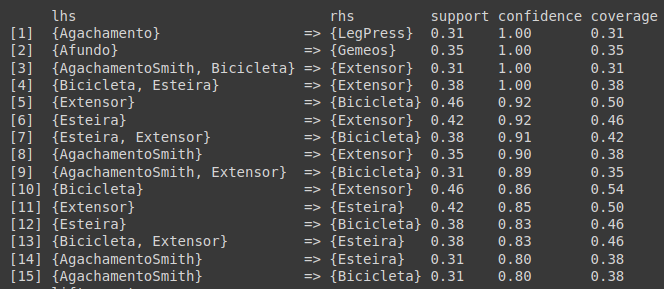
\includegraphics[width=\linewidth]{apendices/fig/8_IAA008_17.png}
\end{figure}

\begin{center}
    \textbf{Lista de comandos emitidos}
\end{center}


\begin{lstlisting}[language=R, style=input]
install.packages('arules', dep=T)
library(arules)
library(datasets)

setwd("/content")
seed_padrao <- 202412

dados <- read.transactions(file="2 - Musculacao - Dados.csv",
format="basket", sep=";")
inspect(dados[1:4])

set.seed(seed_padrao)
rules <- apriori(dados, parameter = list(supp = 0.3, conf = 0.75,
minlen = 2))
summary(rules)

options(digits=2)
inspect(sort(rules, by="confidence"))
\end{lstlisting}